% Template for ICIP-2019 paper; to be used with:
%          spconf.sty  - ICASSP/ICIP LaTeX style file, and
%          IEEEbib.bst - IEEE bibliography style file.
% --------------------------------------------------------------------------
\documentclass{article}
\usepackage{spconf,amsmath,graphicx}
\usepackage[style=IEEE]{biblatex}
\usepackage{multirow}
\usepackage{float}
\usepackage{hyperref}
\addbibresource{lib.bib} % note the .bib is required

% Example definitions.
% --------------------
\def\x{{\mathbf x}}
\def\L{{\cal L}} 
% Title.
% ------
\title{Flower Segmentation with U-Net and ResNet}
%
% Single address.
% ---------------
\name{Alfie Rushby}
\address{}
%
% For example:
% ------------
%\address{School\\
%	Department\\
%	Address}
%
% Two addresses (uncomment and modify for two-address case).
% ----------------------------------------------------------
%\twoauthors
%  {A. Author-one, B. Author-two\sthanks{Thanks to XYZ agency for funding.}}
%	{School A-B\\
%	Department A-B\\
%	Address A-B}
%  {C. Author-three, D. Author-four\sthanks{The fourth author performed the work
%	while at ...}}
%	{School C-D\\
%	Department C-D\\
%	Address C-D}
%
\begin{document}
%\ninept
%
\maketitle
%
\begin{abstract}
This paper focuses on using two models to segment a small flower dataset. The first method involves using a simple U-Net architecture, and it achieved good performance, with a slight tendency to over-extend its flower boundaries. The second method uses a pre-trained ResNet model with 18 layers, and uses the first few layers to pre-train a U-net-like network. This method achieves better performance with tighter boundaries, but is noisier in its boundaries.
\end{abstract}

\section{Introduction}
\label{sec:intro}

This paper focuses on the aspect of two attempts to segment flowers in a small dataset called Oxford Flower Dataset \autocite{nilsbackVisualVocabularyFlower2006}. The specific dataset is of around 750 flowers, with various species, where the images themselves each contain one flower. The difficulty, then, is to create a consistent solution to segment these flowers with the background. These flowers have varying viewpoints, colours, lighting, posing, shape, etc, and so the act of 'knowing' what a flower is with so much variance is very difficult.
\section{Literature Review}
\label{sec:format}

This specific dataset has seen classical attempts at segmenting the flowers. The method uses an approximate segmentation with learned distributions for the background and foreground, and then it iterates on improving the foreground segmentation through using a geometric model of what a flower should look like, until it can converge onto some flower segmentation \autocite{nilsbackDelvingDeeperWhorl2010}. This specific method achieved its performance through a rudimentary learning method, which is by using a set of labelled sample images to create 'learned' distributions. 

The method is affine invariant, but is still susceptible to colour/lighting variations. To circumvent this, a deep learning approach can be used to expand on the early uses of learning from data, specifically a U-net \autocite{ronnebergerUNetConvolutionalNetworks2015}. This expands on the principle by iteratively learning a set of filters that extract progressively more abstract features as you go down the first half of the network via lowering spatial information. The idea then is that these features would only encode the flower and background, or something useful, to then be upscaled with another set of filters into an output segmentation, specifically with up-convolutions.

This method removes the need for any assumptions on how a flower is structured, as the entire 'structure' and the concept of a 'flower' is learnt in the fast half. The only downside with this method is its dependence on data, where the quality and quantity of this data affects the performance to a great extent. 

Another method, SegNet \autocite{badrinarayananSegNetDeepConvolutional2017}, exists, with the main differentiator being that it doesn't use convolutions to upscale directly, and uses pooling indexes to help with the upsampling. This isn't as popular as U-Net because it isn't as direct in learning the upscaling sequence with convolutions. 

All of these methods requires data, and the learning of the encoder section (the downsampling that lowers the spatial resolution progressively) is similar to any classification CNN, like AlexNet or ResNet \autocite{krizhevskyImageNetClassificationDeep2012,heDeepResidualLearning2016}. Training these networks often uses methods like Batch Normalization, which prevents neuron outputs from spiralling into massive values \autocite{ioffeBatchNormalizationAccelerating2015}, and Dropout, which make the network more robust and lessen overfitting by disabling parts of the network during training \autocite{srivastavaDropoutSimpleWay2014}. 

Smaller dataset training in particular has popular configurations for maximizing training efficiency. Along with what has been spoken of, Data Augmentation is another method to expand the dataset by applying affine transformations, along with possible colour variations. This has been shown to reduce overfitting \autocite{shortenSurveyImageData2019} by increasing the model's generalization (through a larger dataset).

These methods can be used together in specific ways to maximize the usefulness in small dataset applications, where the additional concept of injecting this data augmentation technique in the middle of training can maximize its effectiveness \autocite{thanapolReducingOverfittingImproving2020}. 

It is also possible to transfer learn, or fine tune pre-trained models to use their more general convolutions in the encoder as a boost in training, where a pre-trained set of weights for the down-convolution can help it lock into a useful area of search on the onset. It has been shown that pre-training helps with generalizing performance by finding a better 'minima' in loss \autocite{pmlr-v9-erhan10a}.


\section{Methodology}


\subsection{Data pre-processing}

\textbf{Flower Label Mismatch}. There exists flowers without labels, so these are deleted, resulting in 846 labelled flower images to work with.

\textbf{Image Labelling.}  The dataset by default has more than 2 labels for the segmentation, and has a number of flowers that are unlabelled. The possible classes for the labelled pixels are null, flower, background, leaves, and sky. Null and flower are often just the inner flower and its boundary, which can be combined. The other labels are all 'background' and can also be combined into the background class. 

These two modifications have been directly applied to the dataset with MATLAB and saved so that it doesn't need to be re-applied on every run of training.

\textbf{Dataset Split.} The dataset is split to 60:20:20, with it being the training, validation and testing set respectively, using random shuffling.

\textbf{Image Resizing.} For the transfer learning method, it is also important to note that the images and labels will be resized to 224x224 to fit the ResNet input dimension. This is done with MATLAB's resize algorithm.

\textbf{Image Noise.} The images of the flowers are also noisy due to the resizing algorithm used, and so a minor blur has been applied to smooth out the artefacts. 

\begin{figure}[H]
    \centering
    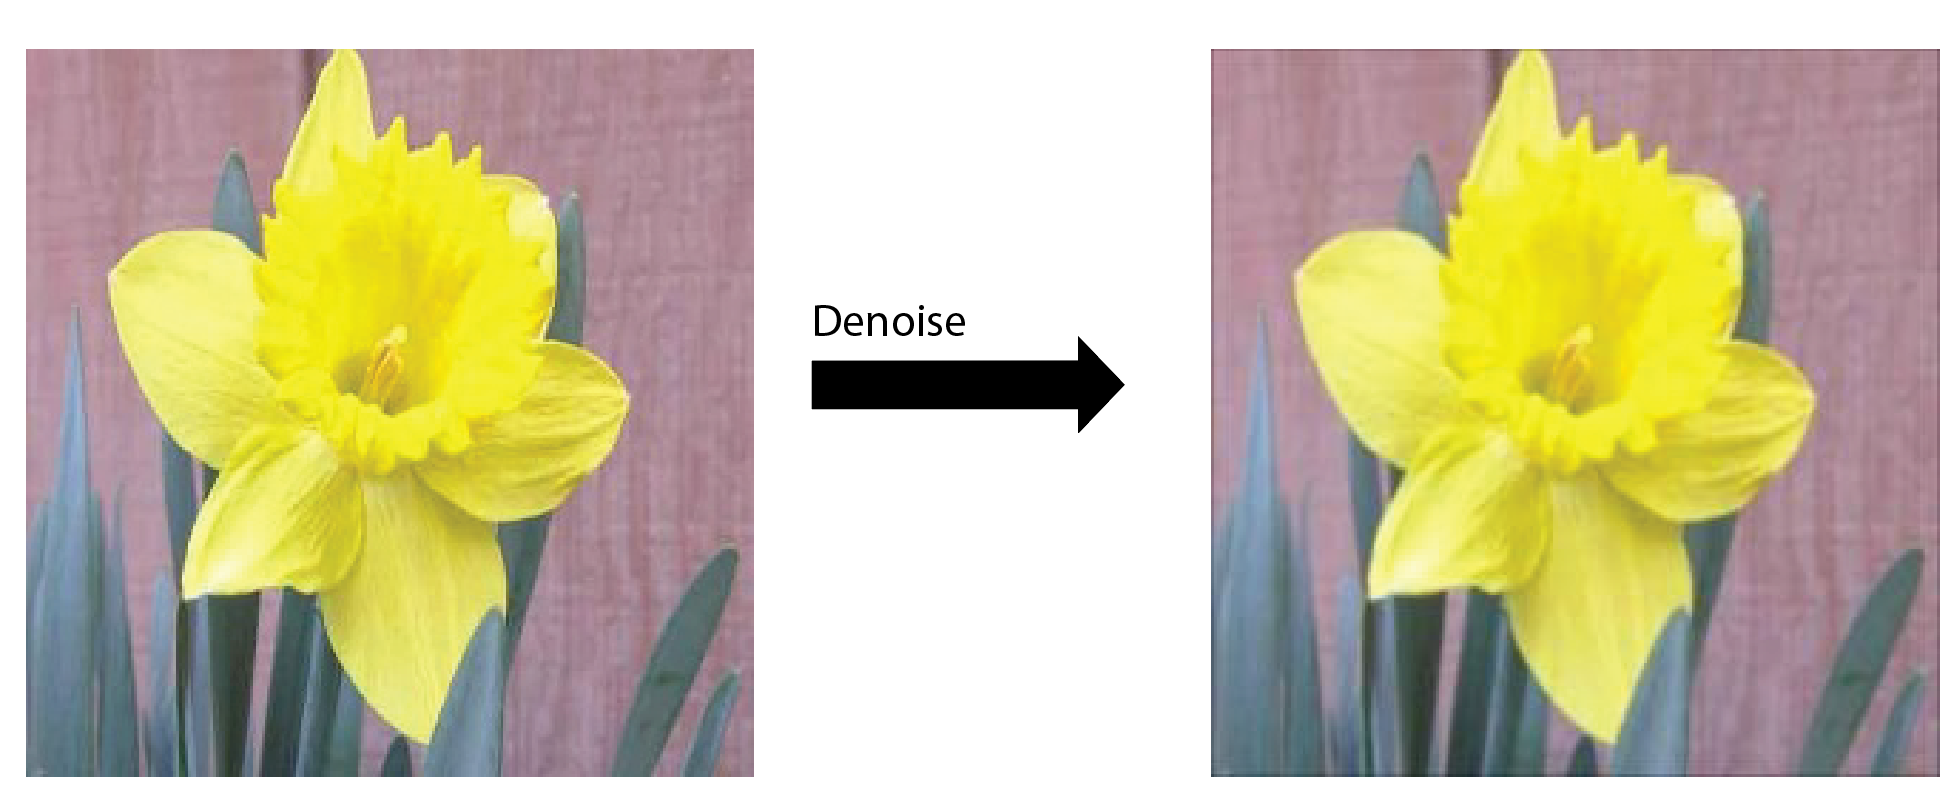
\includegraphics[width=\linewidth]{denoise.png}
    \caption{Denoising of an image in the dataset}
    \label{fig:enter-label}
\end{figure}

This method does add a blur to the image, but it smooths out the artefacts which seems to favour the training if you look at the \textbf{Evaluation} section.


\textbf{Data Augmentation}. Along with pre-processing, an active data augmentation method has been utilized during training, where a set of random affine transformations are applied to the images. This includes X and Y translations between -10 and 10 pixels, an X reflection, and a random scaling factor between 1 and 1.5.

\subsection{Segmentation with a 'from scratch' model}

From what has been discussed in the literature review, a U-Net along with Batch Normalization and Dropout has been chosen:

\begin{figure}[H]
    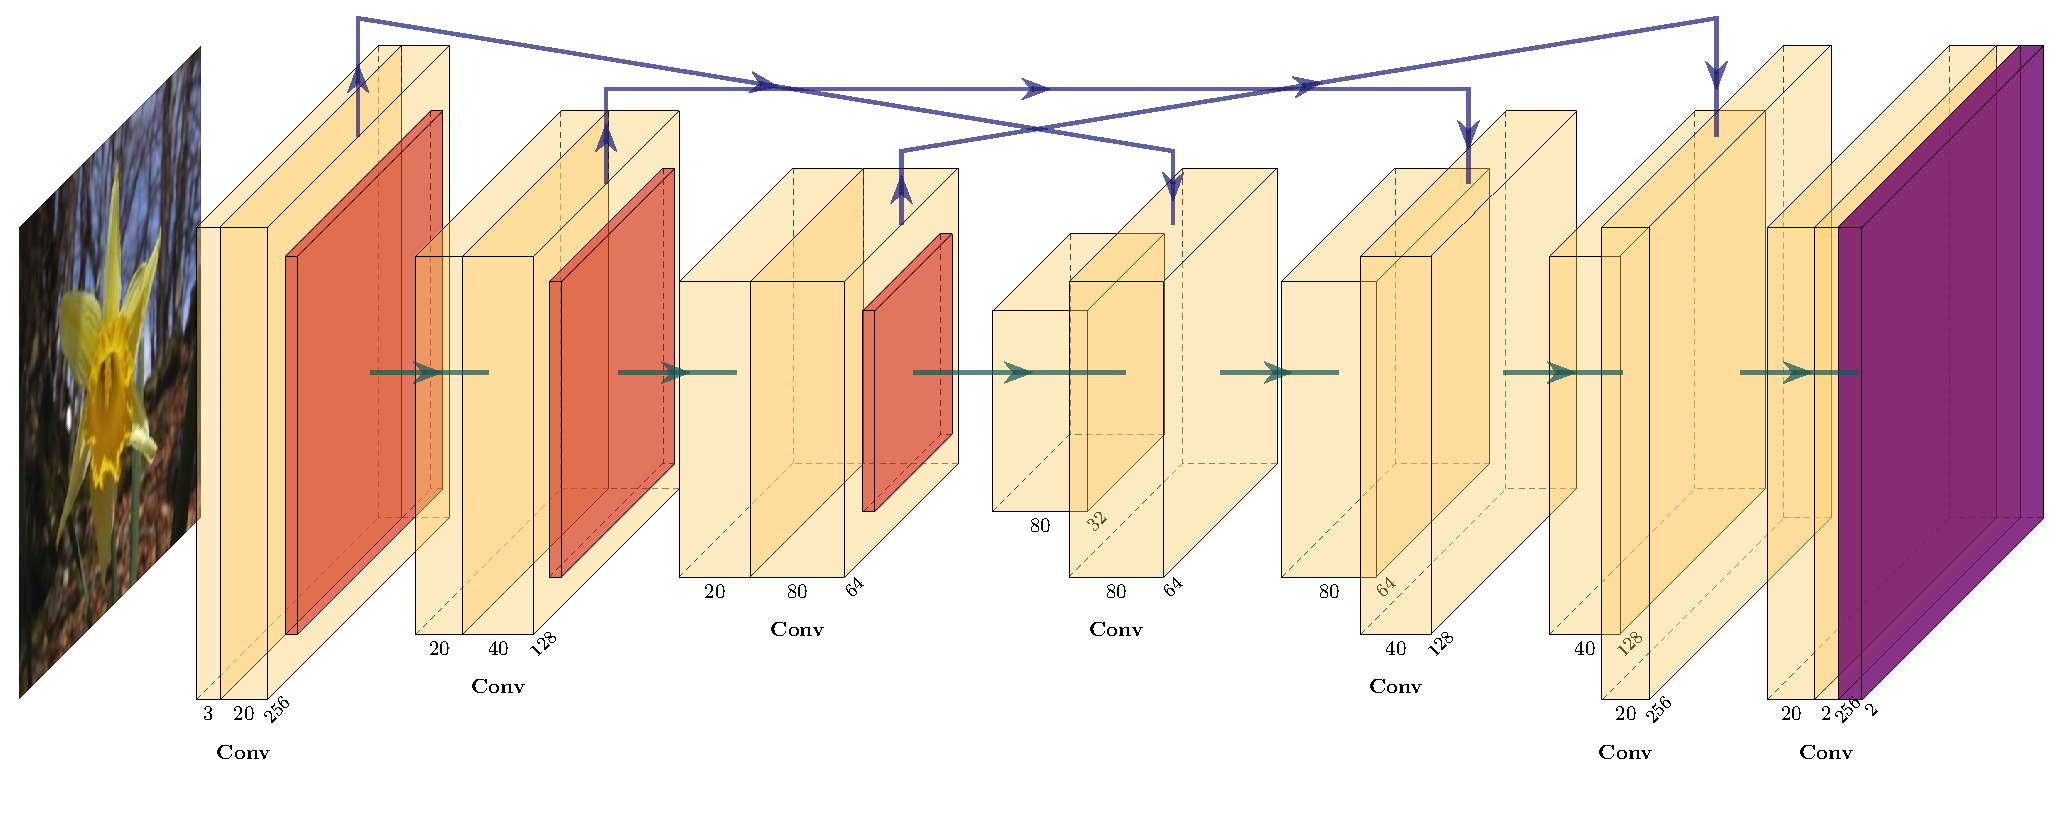
\includegraphics[width=\linewidth]{unet.pdf}
    \caption{Proposed U-Net Model Architecture}
\end{figure}

Relu and batch-normalization layers have been left out of the diagram to save space, but you can assume that every up-convolution has a batch-normalization and every convolution has a ReLu layer.

The network was trained with a maximum epoch of 256, with a linear learning rate of 0.001 with the 'Stochastic Gradient Descent with momentum' optimizer. The simple method was chosen so that a focus could be put on the architecture, as there was not a need for optimizing the time taken to train for such a small model.

\begin{figure}[H]
    \centering
    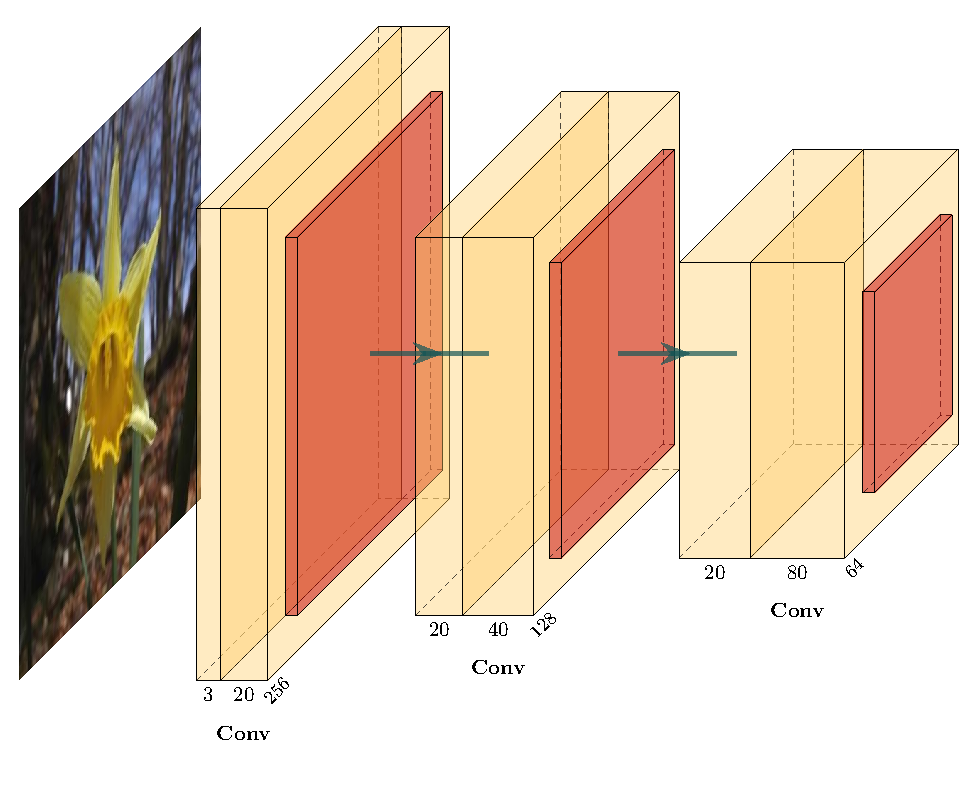
\includegraphics[width=\linewidth]{unetEncode.pdf}
    \caption{U-Net Encoder Architecture}
\end{figure}

The encoder has been set up to start by creating 20 filters from the first convolution, without decreasing the spatial resolution. From this, it follows the pattern of doubling the filters and halving the resolution to 32x32 pixels. 

No more layers were added as it added complexity and made training difficult. It uses 3x3 filters all the way through, with the lowering spatial resolution negating the need for larger ones.

\begin{figure}[H]
    \centering
    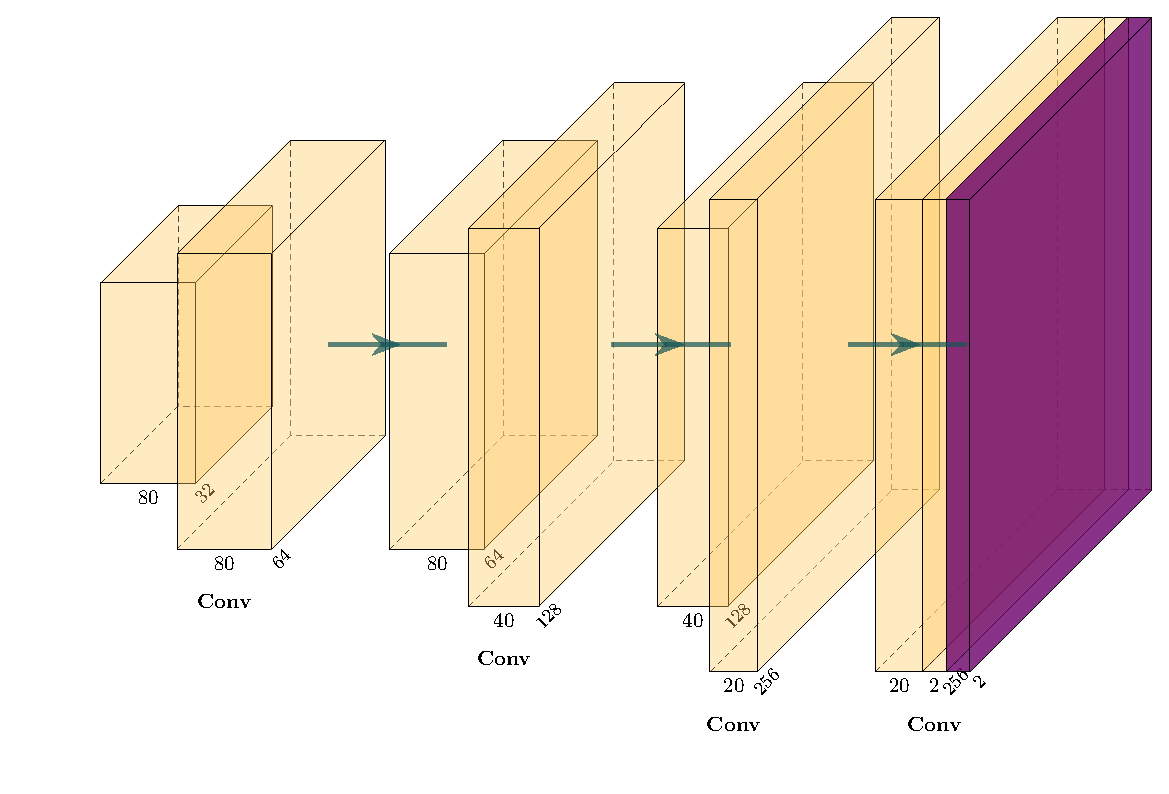
\includegraphics[width=\linewidth]{unetDecode.pdf}
    \caption{U-Net Decoder Architecture}
\end{figure}

The decoder works similarly, except that it uses convolutions to upscale, not max-pooling. The end layer is a softmax layer. It uses 4x4 filters.

\subsection{Segmentation with a 'Pre-trained' model}

Resnet-18 \autocite{resnet18} was used as the base to pre-train off of. This was chosen because it is a relatively small classifier trained on a 1000 class image dataset \autocite{heDeepResidualLearning2016}. It is hypothesized that the first few layers are useful from this to fine tune towards the flower segmentation problem. 

\begin{figure}[H]
    \centering
    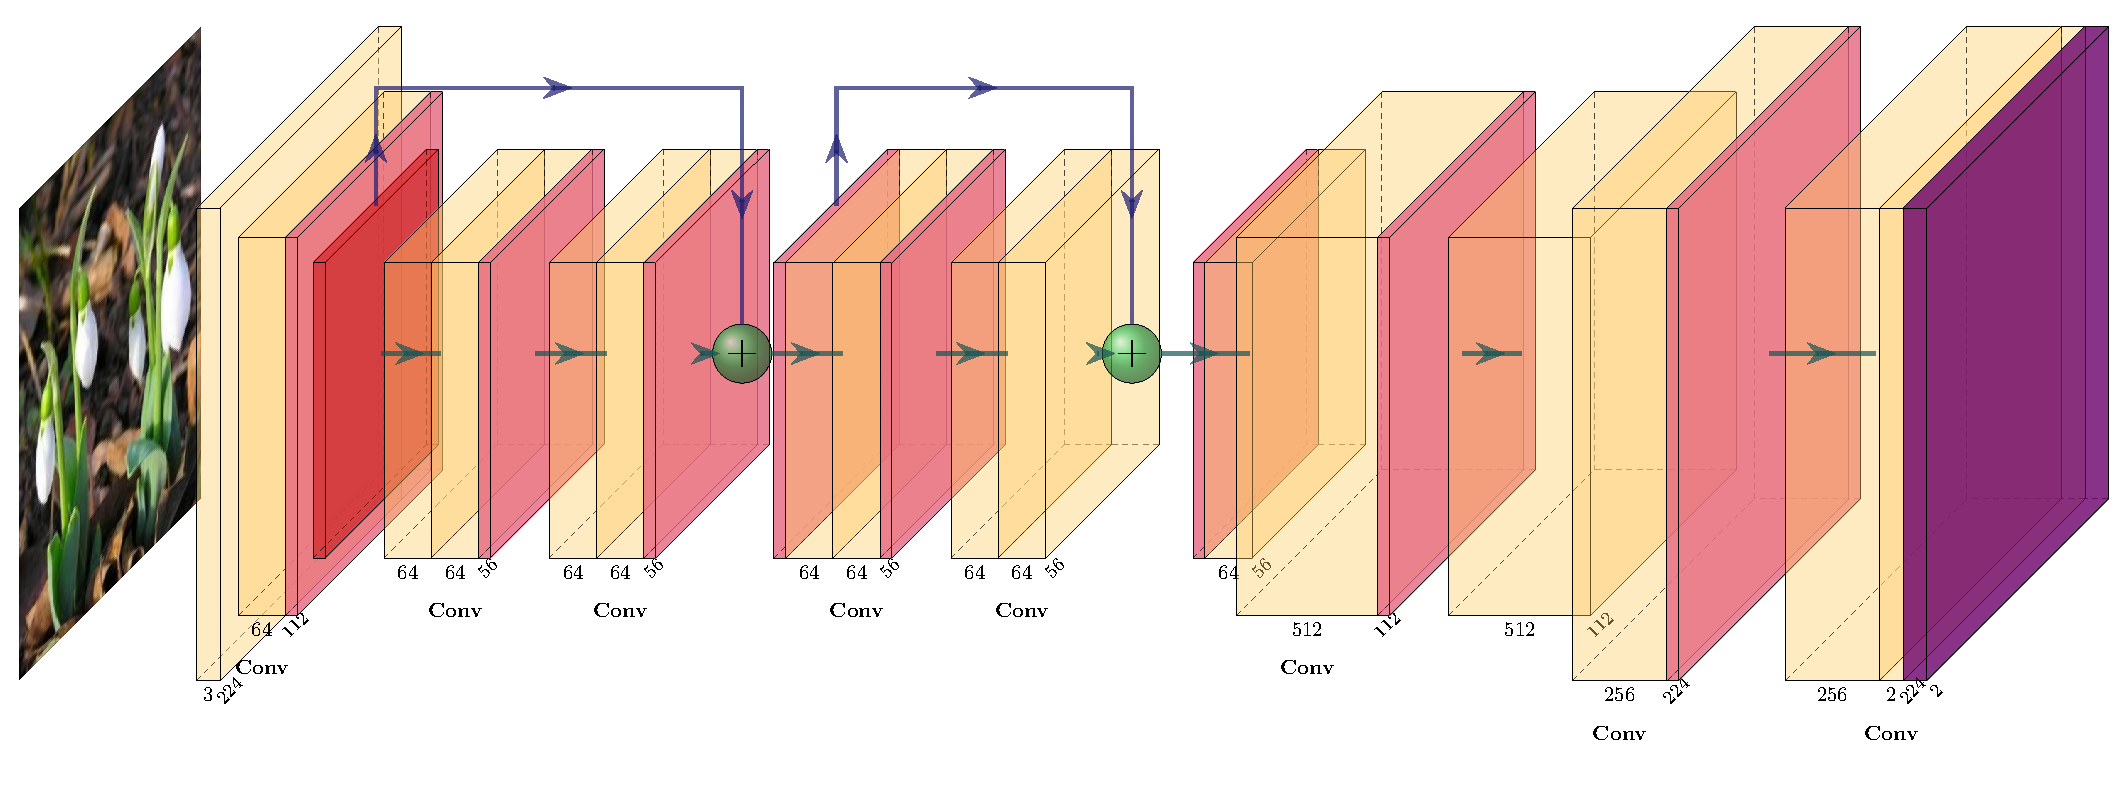
\includegraphics[width=\linewidth]{resnetUnet.pdf}
    \caption{Proposed ResNet + U-Net Model Architecture}
\end{figure}

As ResNet is a classifier a number of modifications were done to make it segment images. A number of the ResNet convolutions were removed to make training easier, leaving just two sets of branched 'layers'. The pink layers are ReLu layers, and they are included because they hold a more important role here. Batch Normalization is not shown, but appears after every convolution in the downsample area. The U-Net skip connections can be assumed.

Most of the ResNet layers were removed to save on training time and memory, as the model did not show any signs of improving without removing most layers.

An interesting quirk from this is that there is only one pooling of downsampling, which is at the start. It also halves the resolution at the start with a convolution. This is due to removing the ResNet layers past the 2 pairs of convolutions.

\begin{figure}[H]
    \centering
    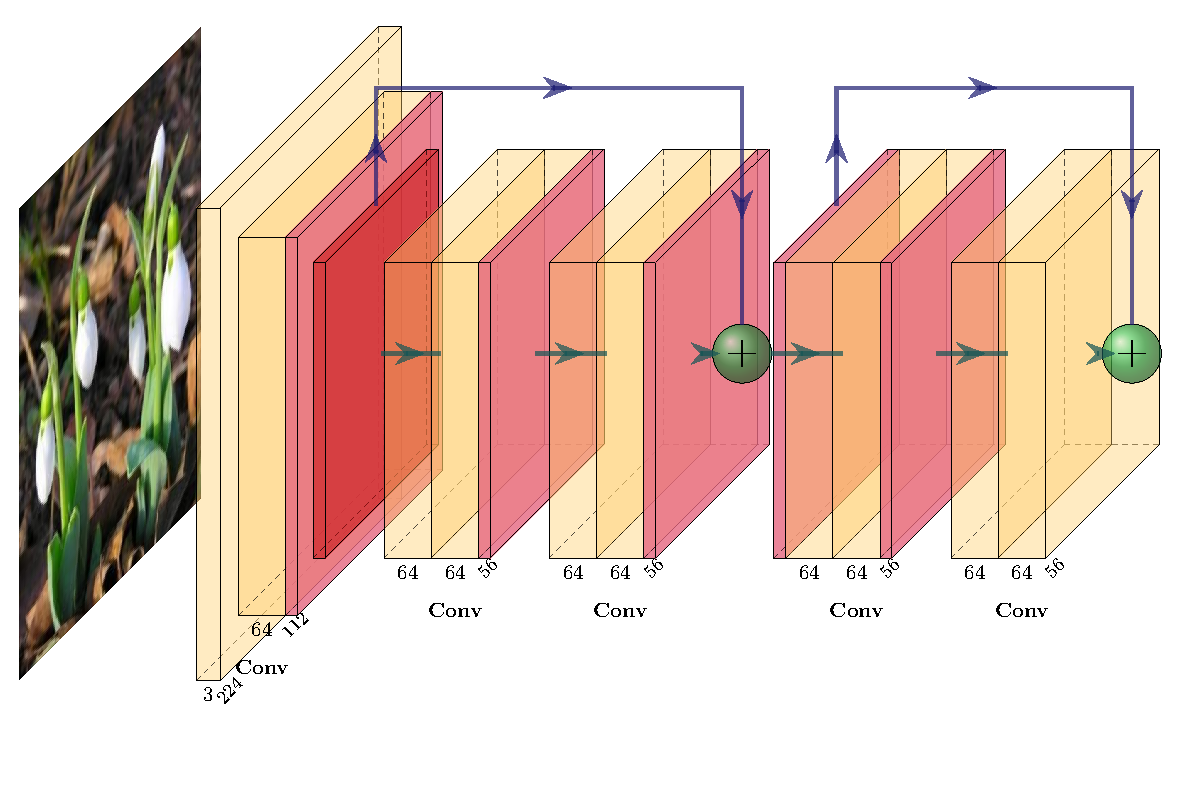
\includegraphics[width=\linewidth]{resnetUnetEncode.pdf}
    \caption{ResNet + U-Net Encoder Architecture}
\end{figure} 

There are two skip connections that sum the previous convolution outputs, where it is done in pairs. This part is taken from ResNet-18 and is pre-trained.

When training, the learning rate of these layers was set to 0.4. Instead of stopping learning completely, a smaller learning rate will allow the training to adapt the first layers, and with the fact that they are already trained from another dataset, gain an advantage when learning.

\begin{figure}[H]
    \centering
    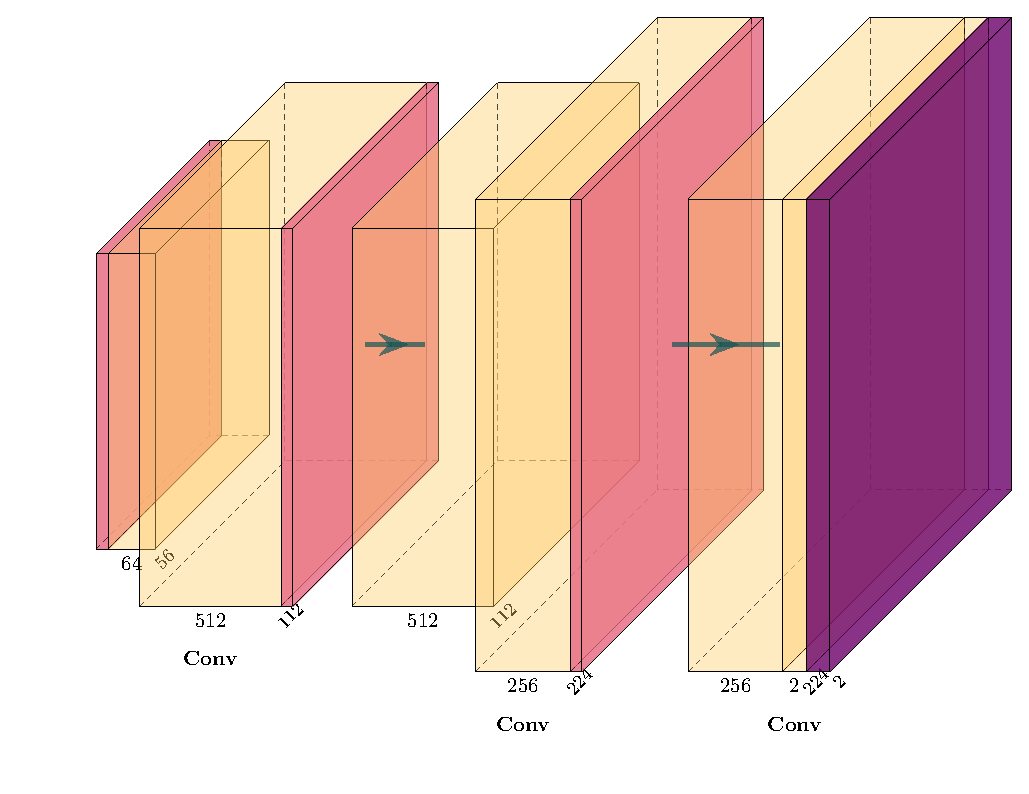
\includegraphics[width=\linewidth]{resnetUnetDecode.pdf}
    \caption{ResNet + U-Net Decoder Architecture}
\end{figure} 

The decoder follows a similar structure to the U-Net used in the 'from-scratch' model. The main difference is there is one less convolution pass, as the dimension inputted to it only requires 2 2x2 filter passes on up-convolutions, from 56x56 to 224x224. The filter sizes were chosen to accommodate the input dimension. All of these layers have initialized weights as they are added onto the ResNet network.

\section{Evaluation \& Discussion}
\label{sec:majhead}

The paper will be comparing the two methods directly. 

\textbf{Evaluation Datasets.}
Evaluation of all methods are done using the Oxford Flower Dataset \autocite{nilsbackVisualVocabularyFlower2006}, on an unseen set of 169 flower images.

\textbf{Implementation Details.}
The model was trained using a GTX 970 GPU, and follows the implementation details show in the methodology. It is set to train for 128-256 epochs and returns the best model according to the validation set's accuracy.

\subsection{'From scratch' model}

\begin{center}
    \begin{tabular}{|c | c  | c |} 
     \hline
     Mean Accuracy & Mean IoU & Mean BF Score \\ [0.5ex] 
     \hline
     90.61\% & 82.44\% & 58.31\% \\ 
     \hline
    \end{tabular}
\end{center}

The high IoU score means it is good at not classifying background pixels as flowers, but its low boundary F1 (BF) contour matching score means that it doesn't align with the true boundary well. It tends to overextend from the flower. 

From this the specific classes are:


\begin{center}
    \begin{tabular}{| c |c | c  | c |} 
     \hline
    Class & Accuracy & IoU & Mean BF Score \\ [0.5ex] 
     \hline
     Flower & 90.01\% & 79.80\% & 46.02\% \\ 
     \hline
     Background & 90.95\% & 85.08\% & 70.60\% \\ 
     \hline
    \end{tabular}
\end{center}

This shows that its major weakness is properly adhering to the flower boundaries as shown with the flower's low BF score.

Its confusion matrix is:

\begin{center}
    \begin{tabular}{| c |c | c |} 
     \hline
    Class  & Flower & Background \\ [0.5ex] 
     \hline
     Flower & 90.13\% & 9.86\% \\ 
     \hline
     Background & 9.04\% & 90.95\%\\ 
     \hline
    \end{tabular}
\end{center}

The confusion matrix shows a rather even confusion with flowers and background. Around 10\% of each class is confused, and this shows there is not a great disparity in its handling of both classes. \textbf{Fig 8} shows this, where it has quite thick boundaries.

\begin{figure}[H]
    \centering
    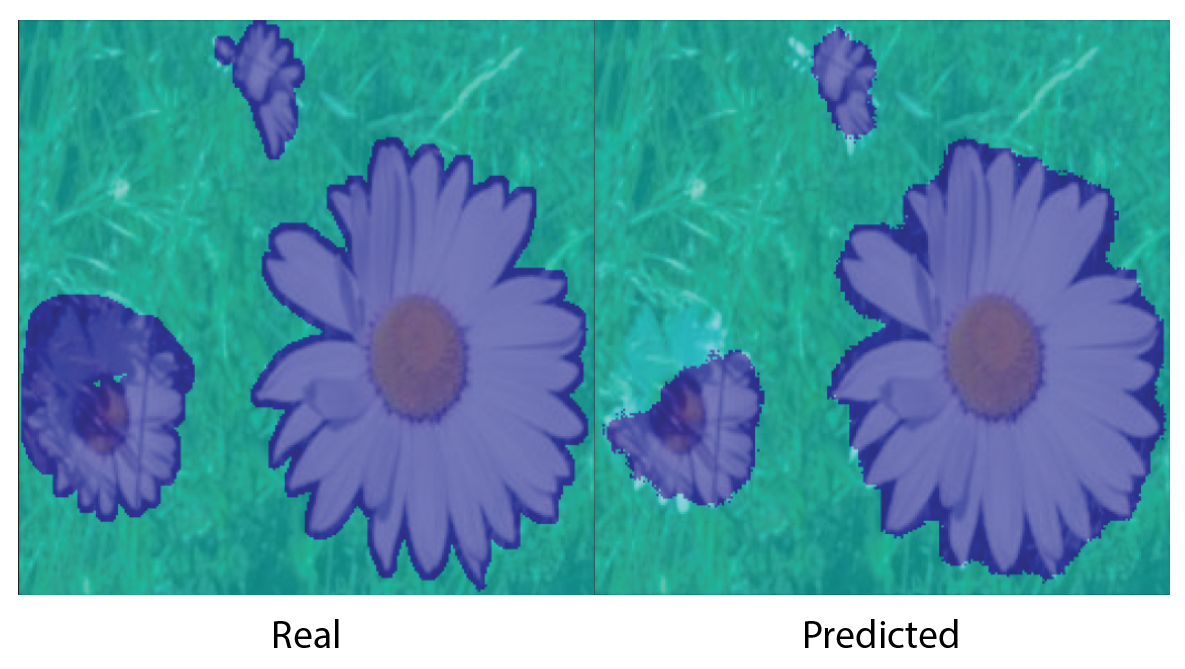
\includegraphics[width=\linewidth]{fromscratchexample.png}
    \caption{Hard Example Image}
\end{figure} 

\subsection{'Pre-trained' model}
\label{sec:print}


\begin{center}
    \begin{tabular}{|c | c  | c |} 
     \hline
     Mean Accuracy & Mean IoU & Mean BF Score \\ [0.5ex] 
     \hline
     92.22\% & 85.2\% & 73.96\% \\ 
     \hline
    \end{tabular}
\end{center}

Compared to the 'from scratch' model it achieves a much higher BF score, along with marginal improvements in average and IoU. This means that it should be much tighter in segmenting the flowers, with less excess boundary.

From this the specific classes are:


\begin{center}
    \begin{tabular}{| c |c | c  | c |} 
     \hline
    Class & Accuracy & IoU & Mean BF Score \\ [0.5ex] 
     \hline
     Flower & 92.94\% & 83.1\% & 67.78\% \\ 
     \hline
     Background & 91.73\% & 87.43\% & 80.147\% \\ 
     \hline
    \end{tabular}
\end{center}

This shows a similar picture, with the BF score improving in both aspects.

Its confusion matrix is:


\begin{center}
    \begin{tabular}{| c |c | c |} 
     \hline
    Class  & Flower & Background \\ [0.5ex] 
     \hline
     Flower & 92.94\% & 7.05\% \\ 
     \hline
     Background & 8.26\% & 91.73\%\\ 
     \hline
    \end{tabular}
\end{center}

 The boundaries are indeed tighter, but a certain amount of noise is present in separated flowers.

\begin{figure}[H]
    \centering
    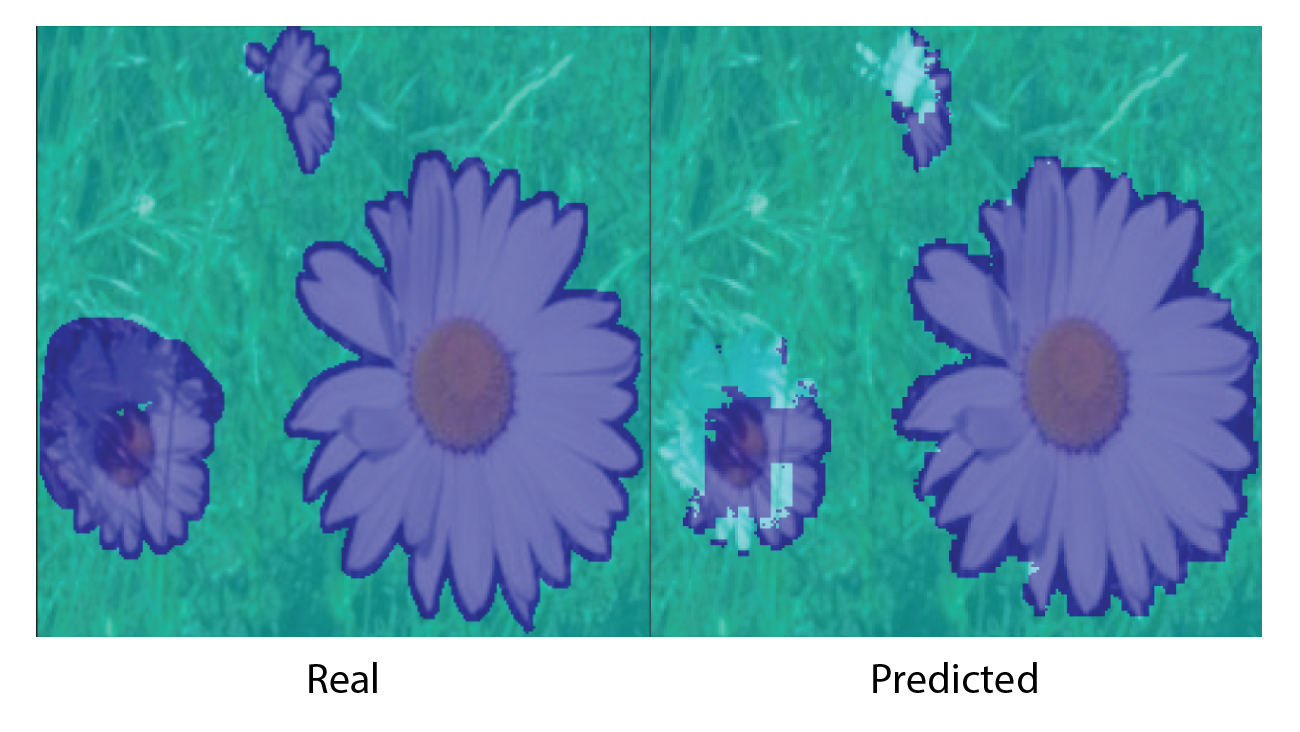
\includegraphics[width=\linewidth]{pretrainedexample.png}
\end{figure} 
An ablation study with the 'from scratch' model shows an improvement with blurring the images to remove noise.
\begin{center}
    \begin{tabular}{| c |c | c  | c |} 
     \hline
    Setup & Mean Accuracy & IoU & Mean BF Score \\ [0.5ex] 
    \hline
      * & 89.90\% & 81.686\% & 58.34\% \\ 
     \hline
     Dropout & 89.86\% & 81.98\% & 57.31\% \\ 
     \hline
     Dropout+Blur & 90.5\% & 82.4\% & 58.31\% \\ 
     \hline
    \end{tabular}
\end{center}

\section{Conclusion}
\label{sec:page}

The pre-trained model performs better in almost all aspects, except for the fact that it is more noisy in certain scenarios. This noise may be due to the ResNet downsampling not removing sufficient spatial resolution. It only pools once with a downsampling convolutional network with the only other layer that lowered spatial resolution being a convolution. This might entail a less abstracted set of filters which can make it more sensitive to image changes.



\section{REFERENCES}

\printbibliography[heading=none]

\end{document}
